\documentclass[a4paper,12pt]{article}
\usepackage{fancyhdr}
\usepackage{graphicx}
\usepackage[utf8]{inputenc}


\title{Design Analysis}
\author{Group Project 3 - Group 2}
\date{March 21 2008}

\begin{document}
\maketitle
\newpage
\tableofcontents
\newpage



\section{Introduction}
This class diagram highlights the classes discovered during the analysis,
and some additional classes discovered during the design of our application.
You will notice than there is no methods in our classes related to the reading,the creation, the deletion or tu updating.
There is no such method because we assume that thoses features are handled from the roots by the GRails Framework.

\section{Class diagram}
\begin{figure}[htbp]
\begin{center}
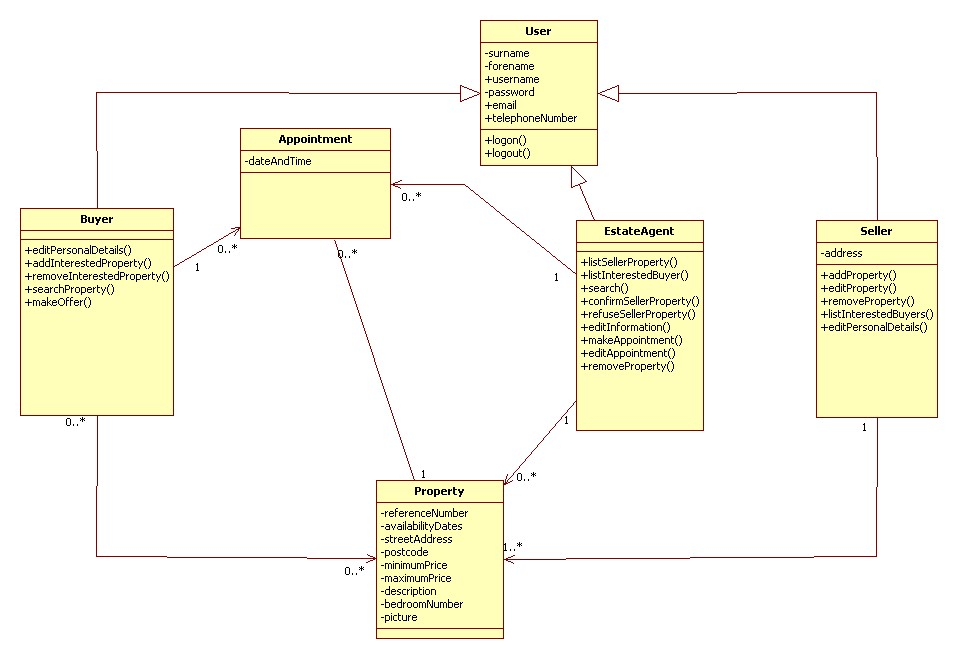
\includegraphics[width=\linewidth]{pics/classDiagram.jpg}
\end{center}
\caption{\footnotesize Class Diagram of Napier Estate Agency}
\end{figure}
\subsection {Classes description}

\subsubsection{EstateAgent class}
An estate agent inherits from an User.
He can :
\begin{itemize}
\item List his properties
\item List the buyers interested by his properties
\item Search a property
\item Validate (or not) a property in order to make it available on the website.
\item Edit the details of a property
\item Set up an appointment
\item Edit an appointment
\item Remove a property
\end{itemize}

\subsubsection{Buyer class}
A buyer inherits from an User.
He can :
\begin{itemize}
\item Add a property to his list of interests
\item Remove a property from this list
\item Search for a property
\item Make an offer to a property
\end{itemize}

\subsubsection{Seller class}
A seller inherits from an User.
He can :
\begin{itemize}
\item Add his property to the website (which is going to be validated by an estate agent)
\item See the list of buyers interested by his properties
\end{itemize}

\subsubsection{User class}
The Seller class, the Buyer class and the EstateAgent class have some common attributes and behaviors,
that's why a parent class, User, as been created to generalize theses attributes and behaviors.
An user is characterized by :
\begin{itemize}
\item His surname
\item His forename
\item A password
\item An email
\item His telephone number (should be formatted like an UK number)
\end{itemize}
This class handles also the login and the logout of an user.

\subsubsection{Property class}
This class describe a property. A property is characterized by : 
\begin{itemize}
\item A reference number (Unique indentifier for a property)
\item A set of availability dates
\item A postcode (constrained by the UK Postcode format)
\item A minimum price
\item A maximum price
\item A short description of the property
\item The number of bedrooms
\item A set of pictures
\end{itemize}

\subsubsection{Appointment class}
This class describe an appointment, set at a particular date and a particular time.
Constraint : A estate agent or a buyer can't have more than one appointment same date.


\end{document}
